\documentclass[a4paper, 14pt]{article}
\usepackage[utf8]{inputenc}
\usepackage[russian]{babel}
\usepackage{graphicx}
\usepackage{listings}
\usepackage{color}
\usepackage{amsmath}
\usepackage{pgfplots}
\usepackage{url}
% подключаем hyperref (для ссылок внутри  pdf)
\usepackage[unicode, pdftex]{hyperref}
\documentclass[a4paper,12pt]{article}
\usepackage[T2A]{fontenc}
\usepackage[utf8]{inputenc}
\usepackage[russian,english]{babel}
\DeclareGraphicsExtensions{.pdf,.png,.jpg,.svg}
\usepackage{titlesec}
\usepackage{caption}
\DeclareCaptionFont{white}{\color{white}} %% это сделает текст заголовка белым
%% код ниже нарисует серую рамочку вокруг заголовка кода.
\DeclareCaptionFormat{listing}{\colorbox{gray}{\parbox{\textwidth}{#1#2#3}}}
\captionsetup[lstlisting]{format=listing,labelfont=white,textfont=white}


\begin{document}
	\begin{titlepage}
		\begin{center}
			\begin{LARGE}
				Отчет по лабораторной работе №1\\
					по курсу "Анализ алгоритмов"\\
					по теме "Расстояние Левенштейна"
			\end{LARGE}
		
			\begin{Large}
				\vspace{10cm}
				Студент: Доктор А.А. ИУ7-53\\
					Преподаватель: Волкова Л.Л.,
								   Строганов Ю.В.\\
				
				\vspace{7cm}2018 г.				   
			\end{Large}
			
		\end{center}
		 
	\end{titlepage}

\tableofcontents
	
\newpage
\section*{Введение}
\addcontentsline{toc}{section}{Введение}

\hspace{1cm}Расстояние Левенштейна (также редакционное расстояние или дистанция редактирования) между двумя строками в теории информации и компьютерной лингвистике — это минимальное количество операций вставки одного символа, удаления одного символа и замены одного символа на другой, необходимых для превращения одной строки в другую\cite{lev_1}.

\hspace{1cm}Впервые задачу упомянул в 1965 году советский математик Владимир Иосифович Левенштейн при изучении последовательностей 0-1. Впоследствии более общую задачу для произвольного алфавита связали с его именем. Большой вклад в изучение вопроса внёс Дэн Гасфилд.

Расстояние Левенштейна и его обобщения активно применяется для исправления ошибок в слове (в поисковых системах, базах данных, при вводе текста, при автоматическом распознавании отсканированного текста или речи); для сравнения текстовых файлов утилитой diff и ей подобными (здесь роль «символов» играют строки, а роль «строк» — файлы); в биоинформатике для сравнения генов, хромосом и белков\cite{lev_2}.
С точки зрения приложений определение расстояния между словами или текстовыми полями по Левенштейну обладает следующими недостатками: при перестановке местами слов или частей слов получаются сравнительно большие расстояния; расстояния между совершенно разными короткими словами оказываются небольшими, в то время как расстояния между очень похожими длинными словами оказываются значительными.\\\\
Расстояние Дамерау — Левенштейна (названо в честь учёных Фредерика Дамерау и Владимира Левенштейна) — это мера разницы двух строк символов, определяемая как минимальное количество операций вставки, удаления, замены и транспозиции (перестановки двух соседних символов), необходимых для перевода одной строки в другую. Является модификацией расстояния Левенштейна: к операциям вставки, удаления и замены символов, определённых в расстоянии Левенштейна добавлена операция транспозиции (перестановки) символов. Расстояние Дамерау-Левенштейна, как и метрика Левенштейна, является мерой "схожести" двух строк. Алгоритм его поиска находит применение в реализации нечёткого поиска, а также в биоинформатике (сравнение ДНК), несмотря на то, что изначально алгоритм разрабатывался для сравнения текстов, набранных человеком (Дамерау показал, что 80\% человеческих ошибок при наборе текстов составляют перестановки соседних символов, пропуск символа, добавление нового символа, и ошибка в символе. Поэтому метрика Дамерау-Левенштейна часто используется в редакторских программах для проверки правописания).

\newpage
\section*{Задачи работы}
\addcontentsline{toc}{section}{Задачи работы}

\begin{enumerate}
\item Изучение алгоритмов Левенштейна и Дамерау-Левенштейна нахождения расстояния между
    строками;
\item Применение метода динамического программирования для матричной реализации указанных
    алгоритмов;
\item Получение практических навыков реализации указанных алгоритмов: двух алгоритмов в
    матричной версии и одного из алгоритмов в рекурсивной версии;
\item Сравнительный анализ линейной и рекурсивной реализаций выбранного алгоритма
    определения расстояния между строками по затрачиваемым ресурсам (времени и памяти);
\item Экспериментальное подтверждение различий во временнóй эффективности рекурсивной и
    нерекурсивной реализаций выбранного алгоритма определения расстояния между строками при
    помощи разработанного программного обеспечения на материале замеров процессорного времени
    выполнения реализации на варьирующихся длинах строк;
\item Описание и обоснование полученных результатов в отчете о выполненной лабораторной
    работе, выполненного как расчётно-пояснительная записка к работе.
\end{enumerate}


	\newpage
	\section{Аналитическая часть}
В этом разделе затронуты темы, описанные ниже.
\begin{enumerate}
\item Определение и формула нахождения расстояния левенштейна.
\item Определение и формула нахождения расстояния Дамерау-Левенштейна.
\item Принцип поиска расстояния для обоих случаев.
\item Применение.
\end{enumerate}
	\subsection{Описание алгоритмов}
	\normalsize \textbf {Расстояние Левенштейна} \\ \normalsize (также редакционное расстояние или дистанция редактирования) между двумя строками в теории информации и компьютерной лингвистике - это минимальное количество операций вставки одного символа, удаления одного символа и замены одного символа на другой, необходимых для превращения одной строки в другую.
    
	Формула, для нахождения расстояния Левенштейна\cite{ifmo_lev}:
	\[
	  D(i,j)=\begin{cases}
	               0\   if\ i == 0, j == 0\\
	               i\   if\ i > 0, j == 0\\
	               j\   if\ i == 0, j > 0\\
	               min\begin{cases}
	               D(s1[1..i],s2[1..j-1]) + 1\\
	               D(s1[1..i-1],s2[1..j]) + 1\\
	               D(s1[1..i-1],s2[1..j-1]) + (S1[i] == S2[j] ? 0 : 1).
	               \end{cases}
	            \end{cases}
	\]
	
    Для нахождения кратчайшего расстояния необходимо вычислить матрицу D, используя вышеприведённую формулу. Её можно вычислять как по строкам, так и по столбцам. Для восстановления редакционного предписания требуется вычислить матрицу D, после чего идти из правого нижнего угла (M,N) в левый верхний, на каждом шаге ища минимальное из трёх значений:
    \begin{itemize}
    \item если минимально (D(i-1, j) + цена удаления символа S1[i]), добавляем удаление     символа S1[i] и идём в (i-1, j);
    \item если минимально (D(i, j-1) + цена вставки символа S2[j]), добавляем вставку     символа S2[j] и идём в (i, j-1);
    \item если минимально (D(i-1, j-1) + цена замены символа S1[i] на символ S2[j]),     добавляем замену S1[i] на S2[j] (если они не равны; иначе ничего не     добавляем), после чего идём в (i-1, j-1)
    Здесь (i, j) — клетка матрицы, в которой мы находимся на данном шаге. Если     минимальны два из трёх значений (или равны все три), это означает, что есть 2     или 3 равноценных редакционных предписания.
	\end{itemize}
	
	Расстояние Дамерау-Левенштейна - это мера разницы двух строк символов, определяемая как минимальное количество операций вставки, удаления, замены и транспозиции (перестановки двух соседних символов), необходимых для перевода одной строки в другую. Является модификацией расстояния Левенштейна: к операциям вставки, удаления и замены символов, определённых в расстоянии Левенштейна добавлена операция транспозиции (перестановки) символов.
	
	Формула, для нахождения расстояния
	\begin{equation}
	Дамерау-Левенштейна\cite{ifmo_dam}:
	
	  D(i,j)=\begin{cases}
	               0\   if\ i == 0, j == 0\\
	               i\   if\ i > 0, j == 0\\
	               j\   if\ i == 0, j > 0\\
	               min\begin{cases}
	               D(s1[1..i],s2[1..j-1]) + 1\\
	               D(s1[1..i-1],s2[1..j]) + 1\\
	               D(s1[1..i-1],s2[1..j-1]) + (S1[i] == S2[j] ? 0 : 1)\\
	               if (i,j > 1) * (S1[i-1] == S2[j]) * (S1[i] == S2[j-1]) D(s1[1..i-2],s2[1..j-2]) + 1\\
	               \end{cases}
	            \end{cases}
	
	\end{equation}
	Для нахождения кратчайшего расстояния необходимо вычислить матрицу D, используя вышеприведённую формулу. Её можно вычислять как по строкам, так и по столбцам. Для восстановления редакционного предписания требуется вычислить матрицу D, после чего идти из правого нижнего угла (M,N) в левый верхний, на каждом шаге ища минимальное из трёх значений:
    \begin{itemize}
    \item если минимально (D(i-1, j) + цена удаления символа S1[i]), добавляем удаление     символа S1[i] и идём в (i-1, j);
    \item если минимально (D(i, j-1) + цена вставки символа S2[j]), добавляем вставку     символа S2[j] и идём в (i, j-1);
    \item если минимально (D(i-1, j-1) + цена замены символа S1[i] на символ S2[j]),     добавляем замену S1[i] на S2[j] (если они не равны; иначе ничего не     добавляем), после чего идём в (i-1, j-1)
    Здесь (i, j) — клетка матрицы, в которой мы находимся на данном шаге. Если     минимальны два из трёх значений (или равны все три), это означает, что есть 2     или 3 равноценных редакционных предписания.
    \item если транспозиция возможна, то возвращаем (D(i-2, j-2) + 1
	\end{itemize}
	
	Данные алгоритмы применяются при поиске информации по запросу, с помощью них можно, найти, если пользователь допустил одну или несколько ошибок в слове, наиболее подходящее(имеющее наименьшее расстояние) к нему слово и заменить его в поисковой строке.  

	
		\newpage
	\section{Конструкторская часть}
	В данном разделе размещены блоксхемы алгоритмов и сравнительный анализ линейной и рекурсивной реализаций
	\subsection{Разработка реализаций алгоритмов}
	
	На рис. \ref{ris:rec} продемонстрирована работа рекурсивного нахождения расстояния Левенштейна


\begin{figure}[ht!]
\center{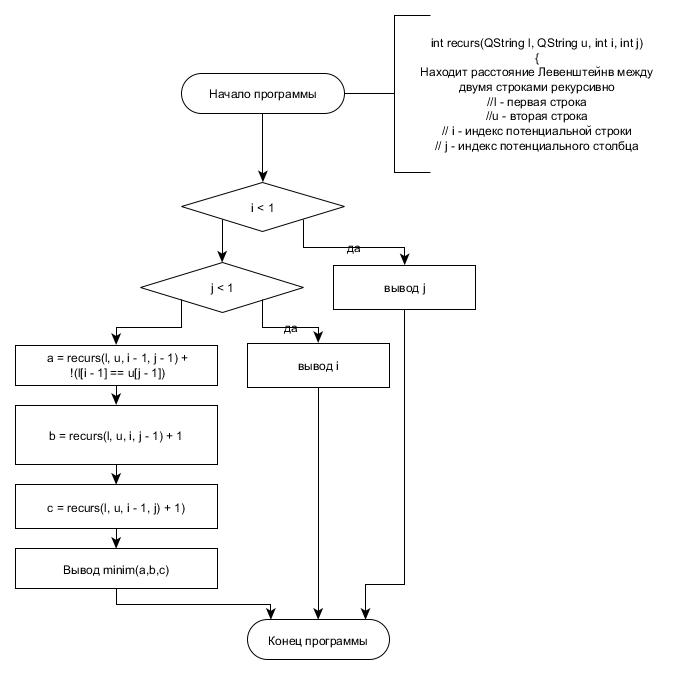
\includegraphics[scale=0.6]{rec.jpg}}
\caption{Рекурсивная реализация нахождения расстояния Левенштейна}
\label{ris:rec}
\end{figure}

	На рис. \ref{ris:matr1} и \ref{ris:matr2} разобрана матричная реализация расстояния Левенштейна

\begin{figure}[pt!]
\center{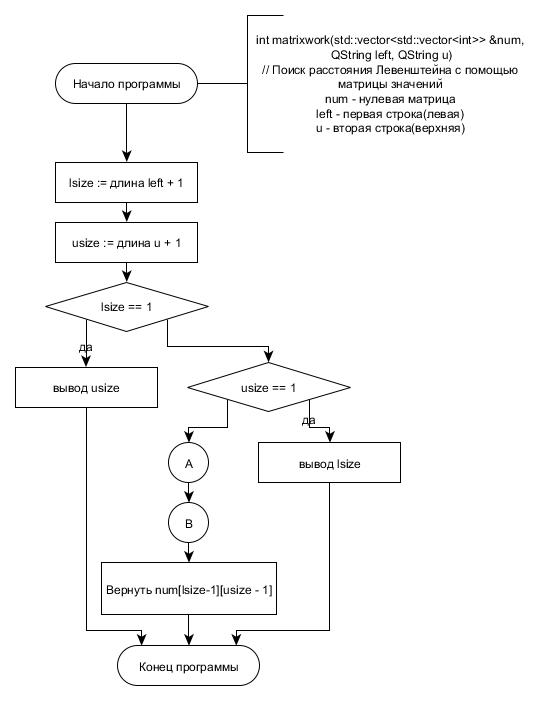
\includegraphics[scale=0.6]{matr1.jpg}}
\caption{Линейный алгоритм поиска расстояния Левенштейна. Часть 1}
\label{ris:matr1}
\end{figure}

\begin{figure}[pt!]
\center{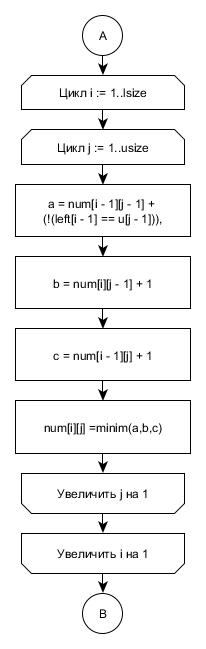
\includegraphics[scale=0.6]{matr2.jpg}}
\caption{Линейный алгоритм поиска расстояния Левенштейна. Часть 2}
\label{ris:matr2}
\end{figure}

\newpage
На рис. \ref{ris:dam1}, \ref{ris:dam2} и \ref{ris:dam3} продемонстрирована работа алгоритма нахождения расстояния Дамерау-Левенштейна. А устройство функции minim указано на рис.  \ref{ris:minim}

\begin{figure}[pt!]
\center{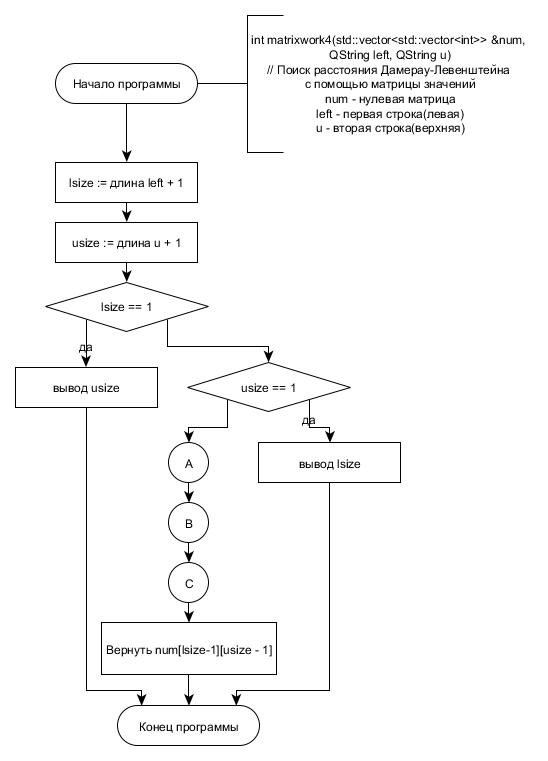
\includegraphics[scale=0.6]{matr4_1.jpg}}
\caption{Линейный алгоритм поиска расстояния Дамерау — Левенштейна.}
\label{ris:dam1}
\end{figure}

\begin{figure}[pt!]
\center{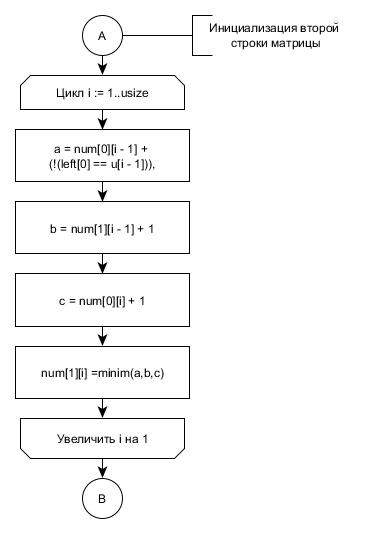
\includegraphics[scale=0.7]{matr4_2.jpg}}
\caption{Линейный алгоритм поиска расстояния Дамерау — Левенштейна.}
\label{ris:dam2}
\end{figure}

\begin{figure}[pt!]
\center{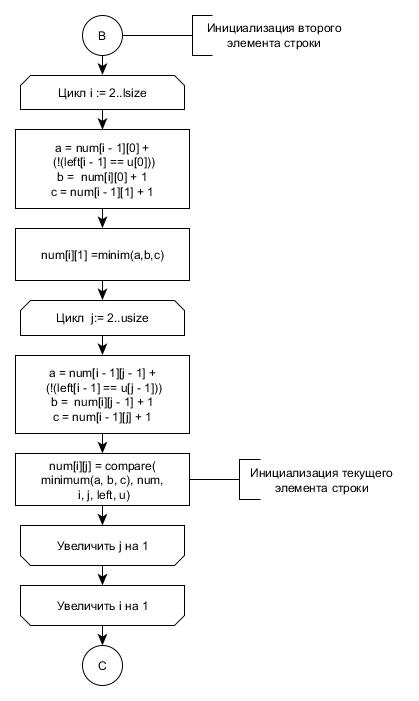
\includegraphics[scale=0.7]{matr4_3.jpg}}
\caption{Линейный алгоритм поиска расстояния Дамерау — Левенштейна.}
\label{ris:dam3}
\end{figure}

\begin{figure}[pt!]
\center{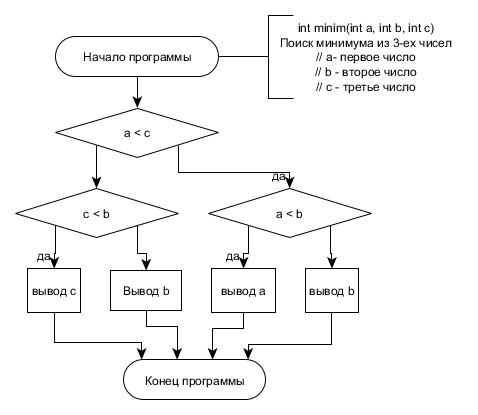
\includegraphics[scale=0.7]{minim.jpg}}
\caption{Линейный алгоритм поиска расстояния Дамерау — Левенштейна.}
\label{ris:minim}
\end{figure}

\newpage
	\subsection{Сравнительный анализ рекурсивной и нерекурсивной реализаций}
	Рекурсивная реализация работает медленнее по сравнение с линейной из-за повторных вычислений, возникающих в ходе работы рекурсивного алгоритма, это наглядно видно на Рис.~\ref{ris:mpr1}, иллюстрирующей дерево рекурсивных вызовов выбранной реализации.Функция rec() принимает на вход 2 строки и 2 индекса, но чтобы не нагружать схему, 2 строки при вызове не подписываются. Для высчитывания цены перехода из диагонального элемента в текущий надо учитывать совпадают ли предыдущие символы строк, но поскольку это не влияет на дерево рекурсии, в схеме я опускаю этот момент и пишу просто число/вызов функции\\
	
	
\begin{figure}[th!]
\center{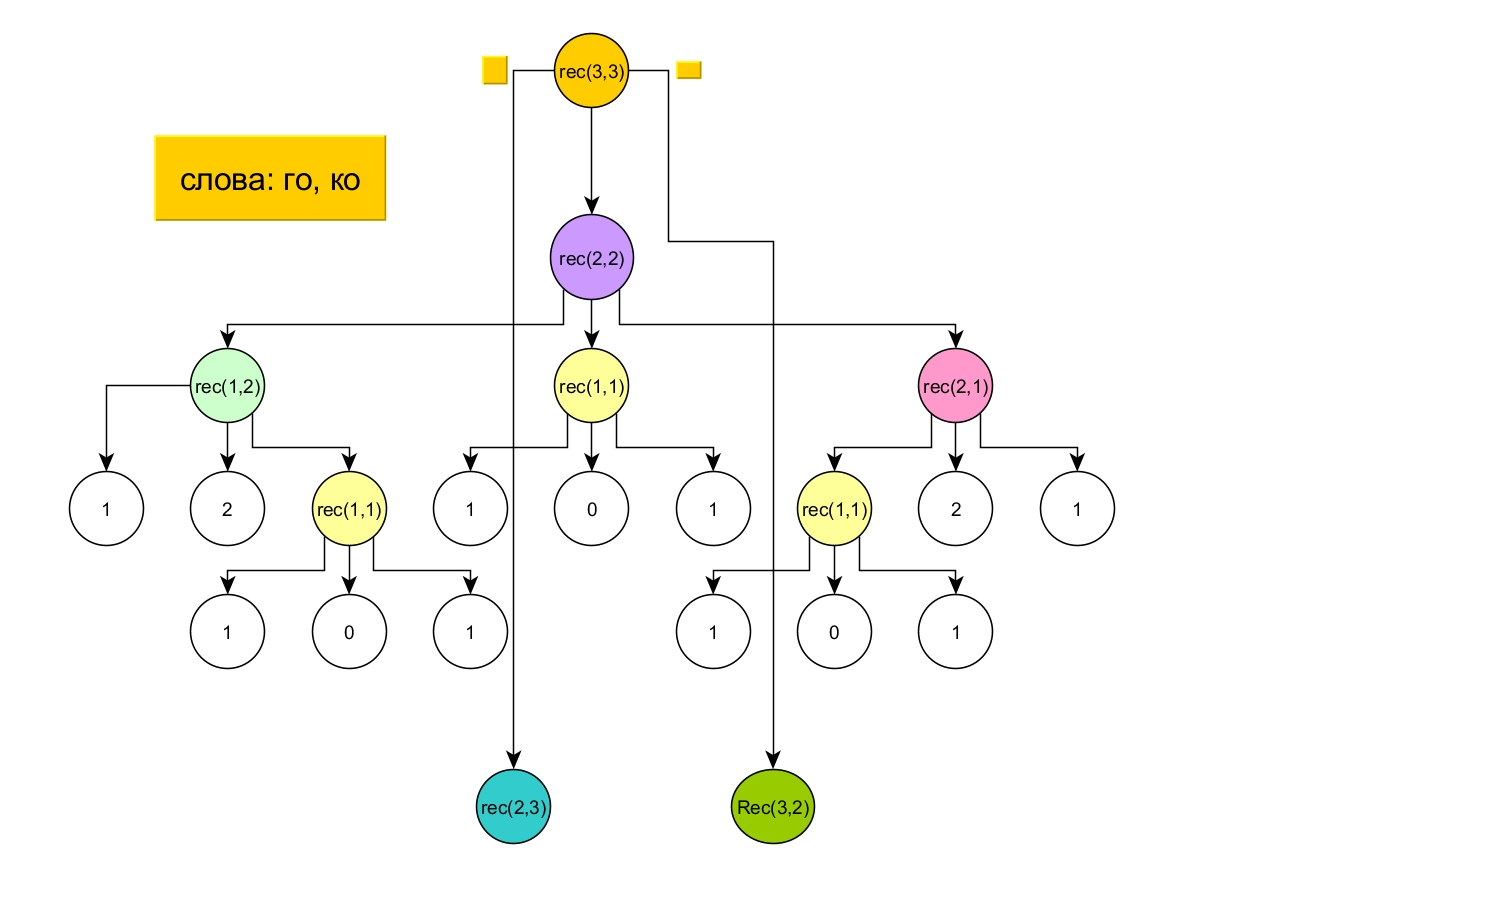
\includegraphics[scale=0.35]{graph1.jpg}}
\caption{Дерево рекурсивных вызовов 1}
\label{ris:mpr1}
\end{figure}

\begin{figure}[pth!]
\center{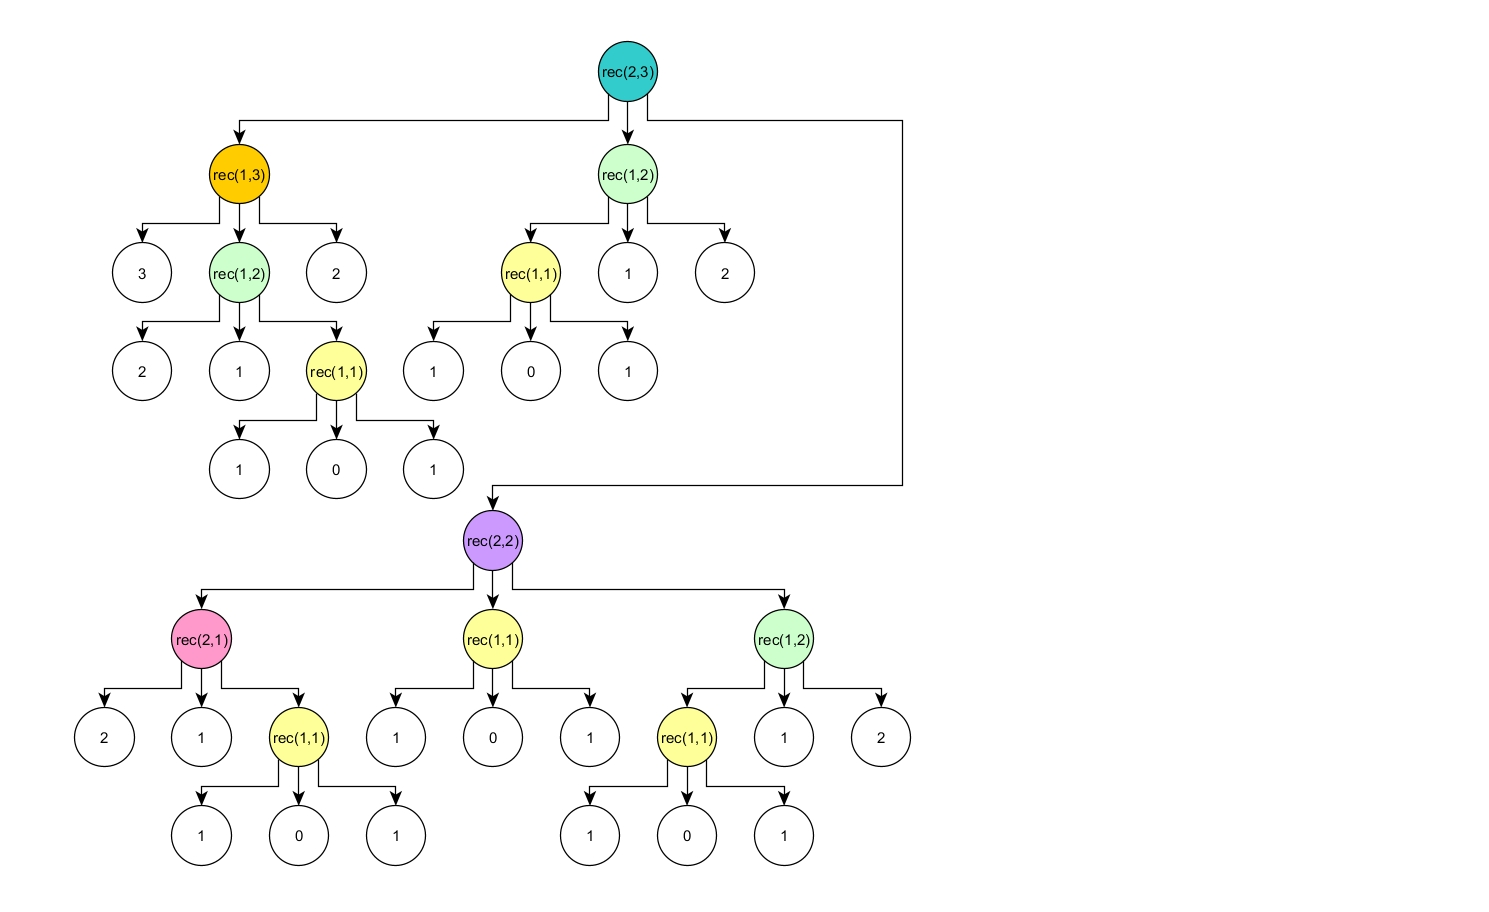
\includegraphics[scale=0.45]{graph2.jpg}}
\caption{Дерево рекурсивных вызовов 2}
\label{ris:mpr2}
\end{figure}

\begin{figure}[pth!]
\center{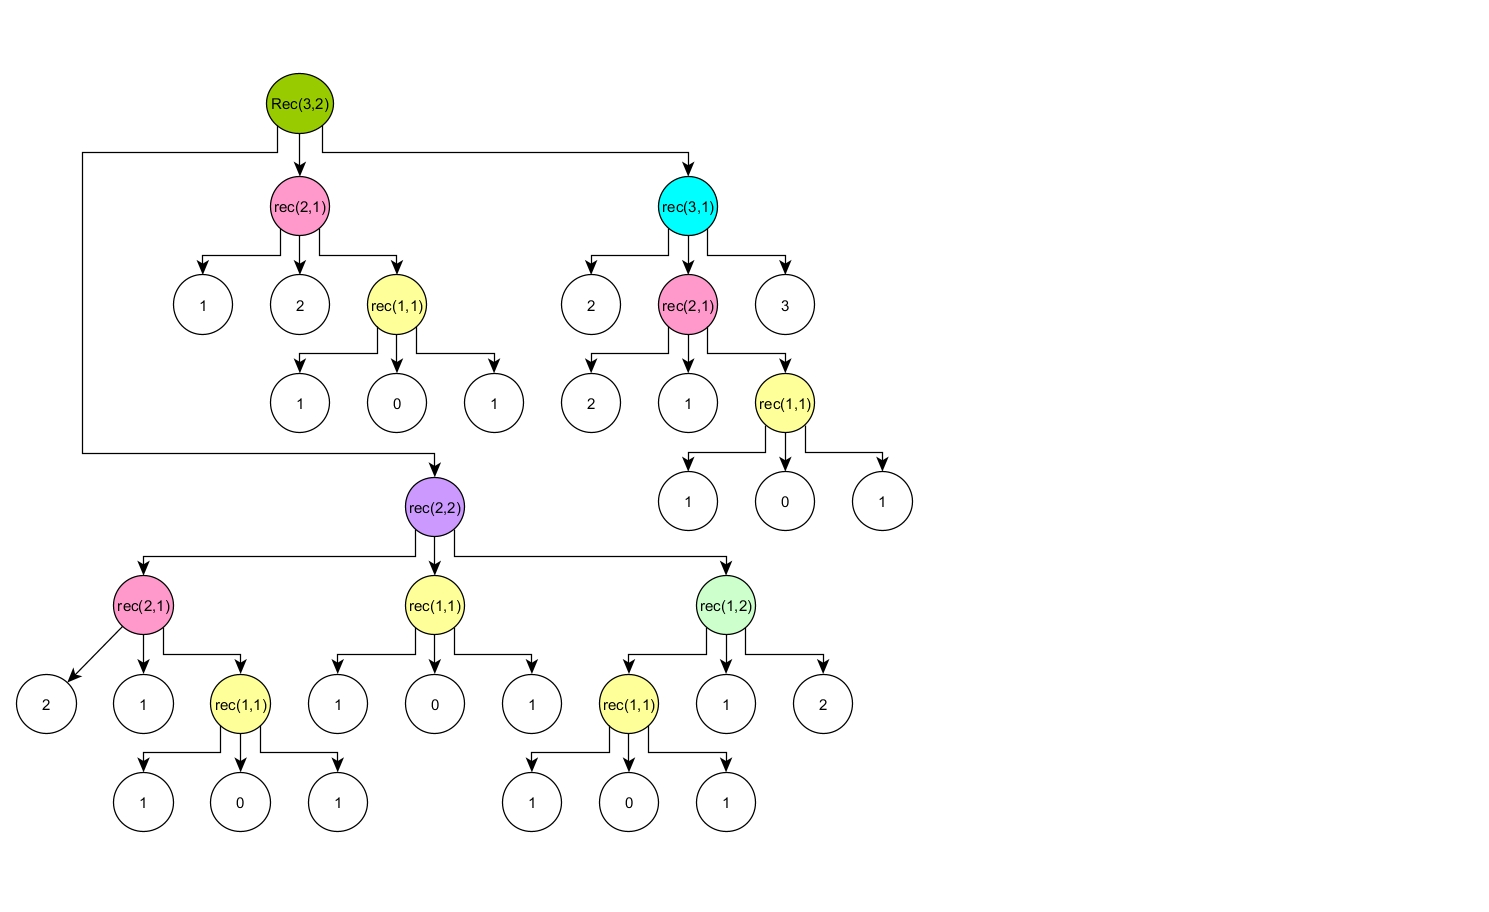
\includegraphics[scale=0.45]{graph3.jpg}}
\caption{Дерево рекурсивных вызовов 3}
\label{ris:mpr2}
\end{figure}
	
	
	\newpage
	\section{Технологическая часть}
	В данном разделе будут приведены требования к программнму обеспечению и средства реализации и листинг кода
	\subsection{Требования к программному обеспечению}
	 Требуется вводить две строки и выводить матрицу и значения расстояний Левенштейна и Дамерау - Левенштейна, полученных различными реализациями (итого 3 шт.). Допускается предоставление двух версий (либо режимов) ПО: для единичного эксперимента и для массовых экспериментов.
	\subsection{Средства реализации}
	Для реализации программ я выбрал язык программирования - C++, так имею большой опыт работы с ним. Среда разработки - Qt. Замеряется время работы процессора с помощью функции:\\
	\lstset{ %
        language=C++,                 % выбор языка для подсветки (здесь это С)
        basicstyle=\small\sffamily, % размер и начертание шрифта для подсветки кода
        numbers=left,               % где поставить нумерацию строк (слева\справа)
        numberstyle=\tiny,           % размер шрифта для номеров строк
        stepnumber=1,                   % размер шага между двумя номерами строк
        numbersep=-5pt,                % как далеко отстоят номера строк от         подсвечиваемого кода
        backgroundcolor=\color{white}, % цвет фона подсветки - используем         \usepackage{color}
        showspaces=false,            % показывать или нет пробелы специальными     отступами
        showstringspaces=false,      % показывать или нет пробелы в строках
        showtabs=false,             % показывать или нет табуляцию в строках
        frame=single,              % рисовать рамку вокруг кода
        tabsize=2,                 % размер табуляции по умолчанию равен 2 пробелам
        captionpos=t,              % позиция заголовка вверху [t] или внизу [b] 
        breaklines=true,           % автоматически переносить строки (да\нет)
        breakatwhitespace=false, % переносить строки только если есть пробел
        escapeinside={\%*}{*)},   % если нужно добавить комментарии в коде
	    keywordstyle=\color{blue}\ttfamily,
	    stringstyle=\color{red}\ttfamily,
	    commentstyle=\color{green}\ttfamily,
	    morecomment=[l][\color{magenta}]{\#},
	    columns=fullflexible
    }
	\begin{lstlisting}[label=time,caption=Функция замера процессороного времени]
    unsigned long long tick(void)
    {
        unsigned long long d;
        __asm__ __volatile__ ("rdtsc" : "=A"     (d));
        return d;
    }
	\end{lstlisting}
	Эта функция в отличие от встроенной функции таймера, способна считать реальное процессорное время работы программы в тиках\cite{lom}.

	\newpage
	\subsection{Реализация алгоритмов}
	
	\begin{lstlisting}[label=matrix-lev,caption=Матричная реализация алгорима Левенштейна]
    std::vector<std::vector<int>> createMatrix(int lsize, int usize)
{
    std::vector<std::vector<int>> matrix;

    std::vector<int> r;
    for (int j = 0; j < usize; j++)
    {
        r.push_back(j);
    }
    matrix.push_back(r);
    for (int i = 1; i < lsize; i++)
    {
        std::vector<int> row;
        for (int j = 0; j < usize; j++)
        {
            row.push_back(0);
        }
        row[0] = i;
        matrix.push_back(row);
    }

    return matrix;
}
	
    int matrixwork(std::vector<std::vector<int>> &num, QString left, QString u)
{
    if (left.size() == 0)
        return u.size();
    if (u.size() == 0)
        return left.size();

    int lsize = left.size() + 1;
    int usize = u.size() + 1;
    for (int i = 1; i < lsize; i++)
    {
        for (int j = 1; j < usize; j++)
        {
            num[i][j] = minim(
                num[i - 1][j - 1] + (!(left[i - 1] == u[j - 1])),
                num[i][j - 1] + 1,
                num[i - 1][j] + 1
            );
        }
    }
    return num[lsize - 1][usize - 1];
}
	\end{lstlisting}
	
	\newpage
	\begin{lstlisting}[label=recur-lev,caption=Рекурсивная реализация алгорима Левенштейна]
    int recurs(QString l, QString u, int i, int j)
{
    if (i < 1)
        return j;
    if (j < 1)
        return i;

    return minim(
        recurs(l, u, i - 1, j - 1) + !(l[i - 1] == u[j - 1]),
        recurs(l, u, i, j - 1) + 1,
        recurs(l, u, i - 1, j) + 1);
}
int minim(int a, int b, int c)
{
    if (a < c)
    {
        if (a < b)
            return a;
        return b;
    }
    if (c < b)
        return c;
    return b;
}
	\end{lstlisting}
	
	\begin{lstlisting}[label=matrix-lev,caption=Матричная реализация алгорима Дамерау-Левенштейна]
	int compare(int a, std::vector<std::vector<int>> &m, int i, int j, QString l, QString u)
{
    int c = a;
    if ((i > 1 && j > 1) && (l[i] == u[j - 1])
        &&
        (l[i - 1] == u[j])
        )
    {
        c = m[i - 2][j - 2] + 1;
    }
    if (c < a)
        return c;
    return a;
}
  int matrixwork4(std::vector<std::vector<int>> &num, QString left, QString u)
{
    if (left.size() == 0)
        return u.size();
    if (u.size() == 0)
        return left.size();

    int lsize = left.size() + 1;
    int usize = u.size() + 1;
    for (int i = 1; i < usize; i++)
    {
        num[1][i] = minim(
            num[0][i - 1] + (!(left[0] == u[i - 1])),
            num[1][i - 1] + 1,
            num[0][i] + 1
        );
    }
    for (int i = 2; i < lsize; i++)
    {
        num[i][1] = minim(
            num[i - 1][0] + (!(left[i - 1] == u[0])),
            num[i][0] + 1,
            num[i - 1][1] + 1
        );
        for (int j = 2; j < usize; j++)
        {
            num[i][j] = compare(minim(
                                    num[i - 1][j - 1] + (!(left[i - 1] == u[j - 1])),
                                    num[i][j - 1] + 1,
                                    num[i - 1][j] + 1
                                ), num, i, j, left, u);
        }
    }
    return num[lsize - 1][usize - 1];
}
	\end{lstlisting}
	
	
	


    \newpage
  \newpage
	\section{Экспериментальная часть}
	В данном разделе будут приведены примеры работы программы, постановка эксперимента и сравнительный анализ алгоритмов на основе экспериментальных данных.
	\subsection{Примеры работы}
	\textbf {Пример 1}\\
	Строка s1 = вилка\\
    Строка s2 = влика\\
    Матрица (расстояние Левенштейна):\\
    0 1 2 3 4 5\\
    1 0 1 2 3 4\\ 
    2 1 1 1 2 3\\
    3 2 1 2 2 3\\
    4 3 2 2 2 3\\
    5 4 3 3 3 2\\
    Матрица (расстояние Дамерау-Левенштейна):\\
    0 1 2 3 4 5\\
    1 0 1 2 3 4\\
    2 1 1 1 2 3\\
    3 2 1 1 2 3\\
    4 3 2 2 1 2\\
    5 4 3 2 2 1\\
    Расстояние Левенштейна\\
    Линейная реализация: 2\\
    Рекурсивная реализация: 2\\
    Расстояние Дамерау-Левенштейна: 1\\\\
    \textbf {Пример 2}\\
	Строка s1 = плитка\\
    Строка s2 = палитра\\
    Матрица (расстояние Левенштейна):\\
    0 1 2 3 4 5 6 7\\
    1 0 1 2 3 4 5 6\\
    2 1 1 1 2 3 4 5\\
    3 2 2 2 1 2 3 4\\
    4 3 3 3 2 1 2 3\\
    5 4 4 4 3 2 2 3\\
    6 5 4 5 4 3 3 2\\
    Матрица (расстояние Дамерау-Левенштейна):\\
    0 1 2 3 4 5 6 7\\
    1 0 1 2 3 4 5 6\\
    2 1 1 1 2 3 4 5\\
    3 2 2 2 1 2 3 4\\
    4 3 3 3 2 1 2 3\\
    5 4 4 4 3 2 2 3\\
    6 5 4 5 4 3 3 2\\

    Расстояние Левенштейна\\
    Линейная реализация: 2\\
    Рекурсивная реализация: 2\\
    Расстояние Дамерау-Левенштейна: 2\\\\
    
    
    \textbf {Пример 3}\\
	Строка s1 = автомобиль\\
    Строка s2 = астронавт\\
    Матрица (расстояние Левенштейна):\\
    0  1 2 3 4 5 6 7 8 9\\
    1  0 1 2 3 4 5 6 7 8\\
    2  1 1 2 3 4 5 6 6 7\\
    3  2 2 1 2 3 4 5 6 6\\
    4  3 3 2 2 2 3 4 5 6\\
    5  4 4 3 3 3 3 4 5 6\\
    6  5 5 4 4 3 4 4 5 6\\
    7  6 6 5 5 4 4 5 5 6\\
    8  7 7 6 6 5 5 5 6 6\\
    9  8 8 7 7 6 6 6 6 7\\
    10 9 9 8 8 7 7 7 7 7\\
    Матрица (расстояние Дамерау-Левенштейна):\\
    0  1 2 3 4 5 6 7 8 9\\
    1  0 1 2 3 4 5 6 7 8\\
    2  1 1 2 3 4 5 6 6 7\\
    3  2 2 1 2 3 4 5 6 6\\
    4  3 3 2 2 2 3 4 5 6\\
    5  4 4 3 3 3 3 4 5 6\\
    6  5 5 4 4 3 4 4 5 6\\
    7  6 6 5 5 4 4 5 5 6\\
    8  7 7 6 6 5 5 5 6 6\\
    9  8 8 7 7 6 6 6 6 7\\
    10 9 9 8 8 7 7 7 7 7\\
    Расстояние Левенштейна\\
    Линейная реализация: 7\\
    Рекурсивная реализация: 7\\
    Расстояние Дамерау-Левенштейна: 7\\\\

    
    \subsection{Постановка эксперимента}
    \hspace{1cm}При сравнении быстродействия алгоритмов были использованы строки длинной в диапазоне от 100 до 1000 с шагом 100. результат одного эксперимента рассчитывался как средний из результатов проведенных испытаний с одинаковыми входными данными.
    Количество повторов каждого эксперимента = 100. Результат одного эксперимента рассчитывается как
    средний из результатов проведенных испытаний с одинаковыми входными данными.
    
    
    \subsection{Сравнительный анализ на материале экспериментальных данных}
    \hspace{1cm}В данном разделе будет проведен сравнительный анализ алгоритмов. График для итеративной реализацией алгоритма изображен на \ref{gr:graph1}. Там же расположен График времени работы рекурсивной реализации изображен на \ref{gr:graph2}
    \newpage
    \begin{table}
        \caption{\begin{center}
         Результаты замеров времени, затрачиваемого итеративной и рекурсивной реализацией алгоритма Левенштейна
        \end{center}}
        \begin{center}
            \begin{tabular}{ | c | c | c | }
                \hline
                Количество символов   &   Время итеративной реализации в тиках&  Время рекурсивной реализации в тиках) \\ \hline  
                    1    &   96    &    102 \\   
                    2    &   175   &    346 \\      
                    3    &   218   &    1695 \\    
                    4    &   300   &    8795\\   
                    5    &   433   &    56628 \\   
                    6    &   651   &    329498 \\   
                    7    &   717   &    1601023\\  
                    8    &   813   &    7545816\\ 
                    9    &   775   &    42556482\\
                    10   &   1039  &   241394895\\
                \hline
            \end{tabular}
        \end{center}
    \end{table}
    \begin{center}График времени работы итеративной реализации алгоритма\end{center}
    \label{gr:graph1}
    \begin{tikzpicture}
		\begin{axis}[
		    %title = График для итеративной реализацией алгоритма,
		    xlabel={Количество символов},
		    ylabel={Время в тиках},
		    ymin = 0, ymax = 5000,
		    legend pos=north west,
		    ymajorgrids=true,
		    grid style=dashed,
		]
  		\addplot[
  		    color=red,
  		    mark=square,
  		    ]
  		    coordinates {
  		    (1,1205)(2,1291)(3,1314)(4,771)(5,844)(6,1172)(7,1141)(8,1966)(9,2096)(10,3101)
  		    };
		    \legend{Линейная реализация Левенштейна}
		\end{axis}
	\end{tikzpicture}

    \newpage
    \begin{center}График времени работы рекурсивной реализации алгоритма\end{center}
    \label{gr:graph2}
    \begin{tikzpicture}
		\begin{axis}[
		    %title = График для итеративной реализацией алгоритма,
		    xlabel={Количество символов},
		    ylabel={Время в тиках},
		    ymin = 0, ymax = 4000000000,
		    legend pos=north west,
		    ymajorgrids=true,
		    grid style=dashed,
		]
  		\addplot[
  		    color=red,
  		    mark=square,
  		    ]
  		    coordinates {
  		    (1,629)(2,3377)(3,19368)(4,102786)(5,575868)(6,3496746)(7,17242107)(8,95848936)(9,548665935)(10,3246981873)
  		    };
		    \legend{Рекурсивная реализация Левенштейна}
		\end{axis}
	\end{tikzpicture}
	
	\newpage
    \begin{table}
        \caption{\begin{center}
         Результаты замеров времени, затрачиваемого итеративной реализацией алгоритма Левенштейна и Дамерау-Левенштейна
        \end{center}}
        \begin{center}
            \begin{tabular}{ | c | c | c |}
                \hline
                Количество символов  &  Время работы Левенштейна в тиках  & Время Дамерау Левенштейна в тиках  \\ \hline  
                    100      &         100320      &         188362  \\
                    200      &         304646      &        731296  \\
                    300      &         639823      &        970084  \\
                    400      &         676468      &        1106100  \\
                    500      &         867839      &       1799650  \\
                    600      &        1050762      &       2690852  \\
                    700      &        1289942      &       3335009  \\
                    800      &        1594564      &       4055009  \\
                    900      &        1692741       &       5494933  \\
                    1000      &       2161930       &         5882436  \\
                \hline
            \end{tabular}
        \end{center}
    \end{table}
    
   \begin{center}График сравнения итеративной реализациии алгоритма Левенштейна и Дамерау-Левенштейна\end{center}
    
    \begin{tikzpicture}
		\begin{axis}[
		    %title = График сравнения итеративной реализациии алгоритма Левенштейна и Дамерау-Левенштейна,
		    xlabel={String length},
		    ylabel={Time in ticks},
		    ymin = 0, ymax = 50000000,
		    legend pos=north west,
		    ymajorgrids=true,
		    grid style=dashed,
		]
		\legend{ 
	        $Levinstein-Damerau$, 
	        $Levinstein$, 
	        }
  		\addplot[
  		    color=red,
  		    mark=square,
  		    ]
  		    coordinates {
  		    (100,433292)(200,1719772)(300,3898057)(400,8803975)(500,10773980)(600,16994409)(700,21872059)(800,31310550)(900,37134388)(1000,46400444)
  		    };

		\addplot[
  		    color=blue,
  		    mark=square,
  		    ]
  		    coordinates {
  		    (100,133546)(200,592935)(300,1315883)(400,3022073)(500,3963211)(600,5175004)(700,6973260)(800,9227619)(900,12293454)(1000,14912271)
  		    %(1,1191)(2,1245)(3,1258)(4,1339)(5,774)(6,2111)(7,1028)(8,2365)(9,2187)(10,2461)
  		    };

		\end{axis}
	\end{tikzpicture}
	
	\hspace{1cm} В результате провденного экспиремента был получен следующий вывод: рекурсивный алгоритм Левенштейна работает гораздо дольше итеративной реализации, начиная с длины строк = 2, время его работы увеличивается в геометрической прогрессии. Итеративный алгоритм значительно превосходит его по эффективности. Алгоритм Дамерау-Левенштейна работает дольше алгоритма Левенштейна, т.к. в нем добавлены дополнительные проверки.
	\newpage
	\section{Заключение}
	\hspace{1cm}В ходе работы были изучены и реализованы в матричной и рекурсивной форме алгоритмы Левенштейна и Дамерау-Левенштейна нахождения расстояния между строками, применены методы динамического программирования для матричной реализации данных алгоритмов. Также был проведен сравнительный анализ линейной и рекурсивной реализаций алгоритма Левенштейна по затрачиваемым ресурсам. Экспирементально подтверждено различие во временноoй эффективности рекурсивной и нерекурсивной реализаций путем замеров процессорного времени работы алгоритмов. Рекурсивный алгоритм Левенштейна работает на несколько порядков медленнее матричной реализации. Если длина сравниваемых строк превышает 10, рекурсивный алгоритм становится неприемлимым для использования.Матричная реализация алгоритма Дамерау-Левенштейна работает дольше алгоритма Левенштейна, т.к. в нем добавлены дополнительные проверки.
    

    \newpage

    \addcontentsline{toc}{section}{Список литературы}
    \begin{thebibliography}{9} 
    \bibitem{lev_1} В. И. Левенштейн. Двоичные коды с исправлением выпадений, вставок и замещений символов. Доклады Академий Наук СССР, 1965. 163.4:845-848. 
    \bibitem{lev_2} Гасфилд. Строки, деревья и последовательности в алгоритмах. Информатика и вычислительная биология. Невский Диалект БВХ-Петербург, 2003. 
    \bibitem{ifmo_lev}https://neerc.ifmo.ru/wiki/index.php?title=\\Задача\_о\_редакционном\_расстоянии,\_алгоритм\_Вагнера-Фишера
    
    \bibitem{ifmo_dam}https://neerc.ifmo.ru/wiki/index.php?title=\\Задача\_о\_расстоянии\_Дамерау-Левенштейна
    
    \bibitem{lom}И.В. Ломовской. Курс лекций по языку программирования C, 2017
    
    \end{thebibliography}

		
		
		
\end{document}